\clearpage{\pagestyle{empty}\cleardoublepage}
\chapter{Architettura del sistema}
%
Il sistema di monitoraggio presentato in questa tesi \`e stato progettato 
quale possibile soluzione per una azienda installatrice di impianti fotovoltaici 
su vasta scala.
%

%
Perch\'e una azienda installatrice dovrebbe interessarsi ad un sistema 
di monitoraggio? Le motivazioni possibili sono almeno due:
%
\begin{itemize}
\item l'azienda potrebbe fornire, ai clienti che lo desiderano, un pacchetto 
      comprensivo di impianto fotovoltaico e sistema di monitoraggio; le 
      informazioni prodotte da quest'ultimo potrebbero essere utilizzate 
      per realizzare un sistema informativo in grado di dare visione 
      al cliente \Item{i} dello stato del suo impianto, \Item{ii} del 
      suo rendimento e, quindi, \Item{iii} del ritorno economico 
      rispetto all'investimento effettuato
%
\item una azienda installatrice fornisce una garanzia sull'impianto e, spesso, 
      si occupa anche della manuntenzione di quest'ultimo; un sistema di 
      monitoraggio permetterebbe di tenere sotto costante osservazione 
      lo stato degli impianti installati, a livello di componente; ci\`o
      permetterebbe una previsione e una identificazione da remoto, di 
      eventuali \emph{fault}, andando ad abbattere i costi di manutenzione
      degli impianti
\end{itemize}
%

%
Nel capitolo precendete sono state presentate alcune delle soluzioni di 
monitoraggio proposte in letteratura. Tuttavia, nessuno dei sistemi analizzati 
\`e stato progettato per un uso impiego su vasta scala da parte di una impresa, 
piuttosto si tratta di sistemi \emph{prototipo}, pensati pi\`u per un uso 
accademico che per la produzione in serie.
%

%
La progettazione di un sistema di monitoraggio da produrre in serie e da utilizzare su 
vasta scala non pu\`o non tenere conto di altri fattori quali il costo dei 
componenti, la facilit\`a d'installazione, ecc.
%

%
La fase iniziale della progettazione del sistema oggetto della presente tesi
ha, quindi, visto l'individuazione della seguente lista di \emph{desiderata}:
%
\begin{itemize}
\item \emph{modularit\`a}, i.e. il sistema deve essere composto da vari dispositivi di 
      campo, ciascuno dei quali con una ben precisa responsabilit\`a; il numero e il 
      tipo dei dispositivi da installare dipender\`a, di volta in volta, dalle dimensioni 
      dell'impianto da monitorare
%
\item \emph{bassi costi di produzione}, i.e. il prezzo del sistema da proporre al cliente 
      finale dovr\`a essere \emph{ragionevolmente} pi\`u basso rispetto al costo totale 
      dell'investimento da lui effettuato
%
\item \emph{semplicit\`a di installazione}, i.e. il sistema dovrebbe richiedere una quantit\`a
      di lavoro minimale per il suo setup; tale obiettivo pu\`o essere raggiunto, ad esempio,  
      progettando un sistema che non richieda l'installazione di troppi cavi per 
      l'interfacciamento dei componenti, oppure, ancora, utilizzando dei dispositivi 
      \emph{autoconfiguranti}
%      
\item \emph{indipendenza da una linea dati cablata}, i.e. non tutti gli impianti fotovoltaici
      sono installati in zone urbane, anzi, molti si trovano in zone rurali non raggiunte da linee 
      dati di terra; l'ideale, per un sistema di monitoraggio, sarebbe fare affidamento
      su meccanismo di trasferimento dati via \emph{gsm} e \emph{gprs}.
%
\end{itemize}
%

%
Il passo successivo, il primo vero step \emph{concreto} di progettazione, \`e consistito 
nell'individuazione delle grandezze rilevanti.
%

%
\section{Grandezze rilevanti}
\label{sec:grandezze-rilevanti}
La scelta delle grandezze rilevanti ha, ovviamente, tenuto conto della tipologia di
informazioni da produrre. 
%

%
Tenendo conto delle esigenze di monitoraggio sopra evidenziate, le quali, fondamentalmente, 
fanno riferimento alle classi di utenti \emph{proprietario} e \emph{manutentore} introdotte in 
\cite{kolodenny08}, sono state individuate come rilevanti, per un generico impianto 
caratterizzato dalla seguente configurazione,
%% sono necessarie per la diagnostica
\begin{itemize}
\item $NI$, numero di inverter.
\item $NS_k, k \in \{1, \dots, NI\}$, numero di stringhe dell'inverter $k$.
\item $\eta _{k}, k \in \{1, \dots, NI\}$, rendimento in potenza
  dell'inverter $k$ (rapporto tra
  potenza in uscita e potenza in ingresso).
\item $NP_{j,k}, k \in \{1, \dots, NI\}, j \in \{1, \dots, NS_k\}$, numero
  di pannelli della stringa $j$ legata all'inverter $k$.
\item $\mu _{i,j,k}, k \in \{1, \dots, NI\}, j \in \{1, \dots, NS_k\}, i \in
  \{1, \dots, NP_{j,k}\}$, rendimento in potenza del pannello $i$ della stringa
  $j$ dell'inverter $k$ (rapporto tra  potenza in uscita e irraggiamento).
\item $S _{i,j,k}, k \in \{1, \dots, NI\}, j \in \{1, \dots, NS_k\}, i \in
  \{1, \dots, NP_{j,k}\}, (m^2)$, Superficie del pannello $i$ della stringa
  $j$ dell'inverter $k$.
\end{itemize}
%
le grandezze definite nel seguente schema, il quale non si limita ad elencarle, 
ma definisce anche quali grandezze si \`e deciso di misurare direttamente e 
quali, invece, si \`e deciso di stimare e quali relazioni utilizzare per la
loro stima:
%
\begin{enumerate}
%%
\item Dati Ambientali:
\begin{itemize}
\item $T, (\deg C)$, Temperatura ambiente.
\item $R, (W/m^2)$, Irraggiamento.
\end{itemize}
%%
%%
\item Grandezze da \textbf{misurare} a monte del contatore bidirezionale:
\begin{itemize}
%%
\item$E_O, (KWh)$, Energia attiva totale prodotta.
\item$P_O, (KW)$, Potenza attiva.
\item$PR_O, (KW)$, Potenza reattiva.
\item$V_O, (V)$, Tensione.
\item$I_O, (A)$, Corrente.
\item$PF_O, (adimensionale)$, Sfsamento (power factor o $cos \phi$).
%%
\end{itemize}
%%
%%
\item Grandezze da \textbf{misurare} a valle dell'inverter $k$:
\begin{itemize}
%%
\item$Iout_{k}, (A)$, Corrente generata.
%%
\end{itemize}
%%
%%
\item Grandezze da \textbf{stimare} per l'inverter $k$:
\begin{itemize}
%%
\item$Vout_{k} = V_O, (V)$, Tensione generata.
\item$Pout_{k} = Vout_{k} \cdot Iout_{k}  \cdot PF_O, (KW)$ Potenza
  (attiva) generata
\item$Pin_{k} = \frac{Pout_k}{\eta _k}, (KW)$, Potenza in ingresso
  all'inverter generata dalle stringhe.
%%
\item$Vin_{k} = \frac{Pin_k}{\sum_{j=1}^{NS_k}{Is_{j, k}}}, (V)$, Tensione
  in ingresso all'inverter
  calcolata sulla base della corrente prodotta dalle stringhe.
%%
\end{itemize}
%%
%%
\item Grandezze da \textbf{misurare} a valle della stringa $j, k$:
\begin{itemize}
%%
\item$Is_{j, k}, (A)$, Corrente generata dalla stringa.
%%
\end{itemize}
%%
%%
\item Grandezze da \textbf{stimare} per la stringa $j, k$:
\begin{itemize}
%%
\item$Vs_{j, k} = Vin_{k}, \forall k, (V)$, Tensione generata da ogni stringa.
\item$Ps_{j, k} = Vs_{j,k} \cdot Is_{j,k}, (KW)$, Potenza generata da ogni
  stringa.
%%
\end{itemize}
\end{enumerate}
%

%
\section{Dispositivi di campo}
Per la misurazione diretta delle grandezze individuate nel paragrafo precedente 
sono state individuate 4 classi di dispositivi di campo:
%% porre l'accento sull'uso delle sensor network e di zigbee
\subsection{Power Transponder}
\subsection{Inverter Transponder}
\subsection{String Transponder}
\subsection{Gateway}





\section{Panoramica del sistema}
%
L'architettura generale del sistema \`e rappresentata in figura \ref{architettura-sistema}.
%
\begin{figure}[!h]
\centering
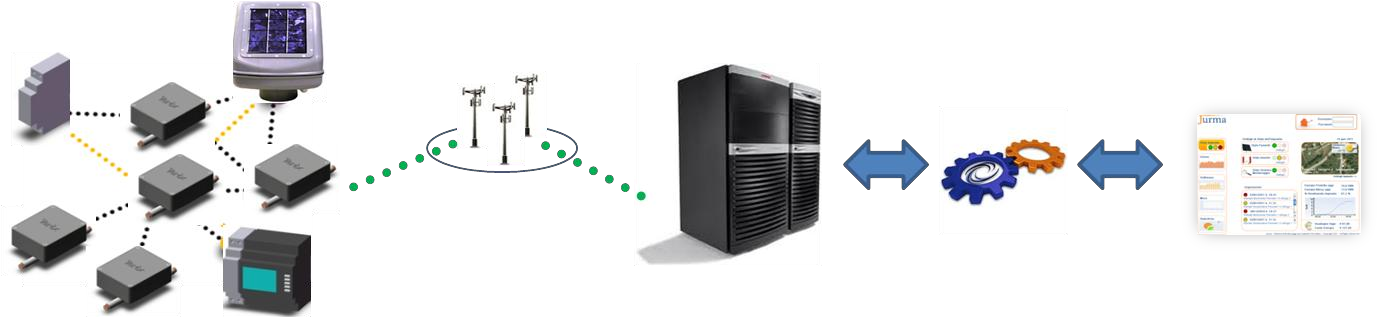
\includegraphics[width=400pt]{img/architecture.png}
\caption{Architettura del sistema}
\label{architettura-sistema}
\end{figure}
%

%







%% misura e stima dei componenti di campo

%%

%%

%% misure rilevate 
%% misure stimate 

%% dopo: come misurare?
%% dispositivi di misura utilizzati
%% sensor network
%% comunicazione over gprs o sms
